\documentclass[usepdftitle=false,usenames,dvipsnames]{beamer}

\usetheme{focus} % see https://github.com/elauksap/focus-beamertheme
% Add option [numbering=none] to disable the footer progress bar
% Add option [numbering=fullbar] to show the footer progress bar as always full with a slide count

\usepackage{booktabs} % Required for better table rules
\usepackage{bm,times,amsmath,mathtools,tabularx}

\usepackage{tikz}
\usetikzlibrary{decorations.pathreplacing,calc}

\usepackage{hyperref}
\hypersetup{
    pdftitle={Kaczmarz iteration}
}

\newcommand{\tikzmark}[1]{\tikz[overlay,remember picture] \node (#1) {};}

\newcommand{\eps}{\epsilon}

\newcommand{\CC}{\mathbb{C}}
\newcommand{\EE}{\mathbb{E}}
\newcommand{\PP}{\mathbb{P}}
\newcommand{\RR}{\mathbb{R}}

\newcommand{\grad}{\nabla}
\newcommand{\Div}{\nabla\cdot}

\newcommand{\cond}{\operatorname{cond}}
\newcommand{\trace}{\operatorname{tr}}
\newcommand{\Span}{\operatorname{span}}

\newcommand{\argmin}[1]{\underset{#1}{\operatorname{arg\, min}\,}}

\newcommand{\hbn}{\hat{\mathbf{n}}}

\newcommand{\ba}{\mathbf{a}}
\newcommand{\bb}{\mathbf{b}}
\newcommand{\bc}{\mathbf{c}}
\newcommand{\be}{\mathbf{e}}
\newcommand{\bbf}{\mathbf{f}}
\newcommand{\bg}{\mathbf{g}}
\newcommand{\bn}{\mathbf{n}}
\newcommand{\br}{\mathbf{r}}
\newcommand{\bu}{\mathbf{u}}
\newcommand{\bv}{\mathbf{v}}
\newcommand{\bw}{\mathbf{w}}
\newcommand{\bx}{\mathbf{x}}
\newcommand{\by}{\mathbf{y}}
\newcommand{\bz}{\mathbf{z}}

\newcommand{\bF}{\mathbf{F}}
\newcommand{\bV}{\mathbf{V}}
\newcommand{\bX}{\mathbf{X}}

\newcommand{\balpha}{\bm{\alpha}}
\newcommand{\bxi}{\bm{\xi}}

\newcommand{\bzero}{\bm{0}}

\newcommand{\rhoi}{\rho_{\text{i}}}

\newcommand{\ip}[2]{\left(#1,#2\right)}

\newcommand{\mR}{R^{\bm{\oplus}}}
\newcommand{\iR}{R^{\bullet}}

\newcommand{\pp}{{\text{p}}}
\newcommand{\qq}{{\text{q}}}
\newcommand{\rr}{{\text{r}}}

\newcommand{\bus}{\bu|_s}

\newcommand{\ds}{\displaystyle}



\title{Kaczmarz iteration}

\subtitle{A 21st century revival?}

\author{Ed Bueler}

\titlegraphic{\vspace{0mm} 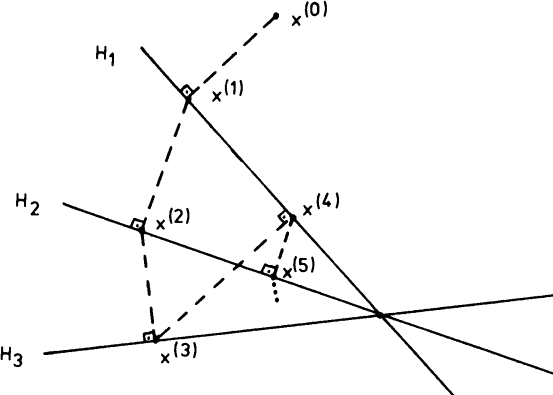
\includegraphics[width=0.55\textwidth]{figs/kaczmarz-censor.png}}

%\institute{University of Alaska Fairbanks}

\date{DMS Colloquium \\ UAF June 2022}


\begin{document}

\begin{frame}
	\maketitle
\end{frame}


\begin{frame}{outline}

\begin{itemize}
\item what is Kaczmarz iteration (1937)?
\item examples, history, geometry, convergence
\item brief survey of classical and Krylov iterations
    \begin{itemize}
    \item[$\circ$] how does Kaczmarz compare?
    \end{itemize}
\item randomized Kaczmarz iteration (2009)
\item a new iterative paradigm (2015):

\begin{center}
\emph{row-centric sketch-and-project}
\end{center}

    \begin{itemize}
    \item[$\circ$] alternative to preconditioned Krylov? probably not
    \end{itemize}
\item connection to machine learning
    \begin{itemize}
    \item[$\circ$] randomized Kaczmarz iteration for \emph{online linear systems}
    \end{itemize}
\end{itemize}
\end{frame}


\begin{frame}{linear systems}

\begin{itemize}
\item start with notation and context
\item to solve: linear systems $A \bx = \bb$ where
    \begin{itemize}
    \item[$\circ$] $A$ is $m\times n$ matrix, $m$ rows and $n$ columns \hfill $\RR^n \stackrel{A}{\to} \RR^m$
    \item[$\circ$] $\bx \in \RR^n$, a column vector
    \item[$\circ$] $\bb \in \RR^m$, a column vector with entries $b_i$
    \end{itemize}
\item $\ba_i$ denotes a \alert{row} of $A$:
    $$A = \left[\begin{array}{c} \, \ba_1 \quad \\ \hline
                                 \, \vdots \quad \\ \hline
                                 \, \ba_m \quad \end{array}\right]$$

    \begin{itemize}
    \item[$\circ$] $\ba_i^\top \in \RR^n$ is a column vector
    \end{itemize}
\end{itemize}
\end{frame}


\begin{frame}{solving linear systems: direct methods}

$$A \bx = \bb$$

\begin{itemize}
\item how expensive is it to solve a linear system?
    \begin{itemize}
    \item[$\circ$] cost $=$ amount of arithmetic
    \item[$\circ$] measured in floating-point operations (flops)
    \end{itemize}
\item standard \emph{direct} algorithms require $O(m^3)$ flops for $A$ square
    \begin{itemize}
    \item[$\circ$] Gaussian elimination (LU), QR decomposition
    \end{itemize}
\item direct methods can't be used for large systems
    \begin{itemize}
    \item[$\circ$] certain $m=10^7,10^8$ systems are now routine on desktops
    \item[$\circ$] \emph{not} by using $O(m^3)=O(10^{24})$ algorithms!
    \item[$\circ$] world's fastest supercomputer does $10^{24}$ flops in a month
    \end{itemize}
\end{itemize}

\bigskip
\hspace{20mm} 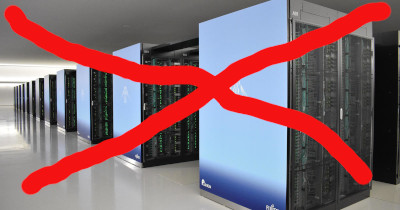
\includegraphics[height=15mm]{figs/fugaku-too-slow}

\vspace{-10mm} \hfill $\gets$ \emph{too slow for direct methods!}
\end{frame}


\begin{frame}{sparsity and iteration}

$$A \bx = \bb$$

\begin{itemize}
\item key practical fact: many matrices are sparse
\item a matrix is \emph{sparse} if it has enough zero entries so that solutions are significantly-faster than $O(m^3)$

{\scriptsize
   $$A = \begin{bmatrix} \bullet & \bullet & \bullet & \bullet & \bullet \\ \bullet & \bullet & \bullet & \bullet & \bullet \\ \bullet & \bullet & \bullet & \bullet & \bullet \\ \bullet & \bullet & \bullet & \bullet & \bullet \\ \bullet & \bullet & \bullet & \bullet & \bullet\end{bmatrix} \hspace{15mm}
   B = \begin{bmatrix} \bullet & \bullet & & & \bullet \\ & \bullet & \bullet & & \\  &  & \bullet & \bullet & \\ \bullet & & & \bullet & \bullet \\ & \bullet & & & \bullet \end{bmatrix}$$

\vspace{-2mm}
$$\qquad \text{dense} \hspace{39mm} \text{sparse}$$
}

\item iterative methods can sometimes take advantage of sparsity to get $O(m)$ or $O(m^2)$ performance
    \begin{itemize}
    \item[$\circ$] especially \emph{preconditioned Krylov} iterations
    \end{itemize}
\end{itemize}
\end{frame}


\begin{frame}{Kaczmarz iteration}

\begin{itemize}
\item viewpoint: \, linear system $A\,\bx=\bb$ is a list of scalar equations

\vspace{-6mm}
    \begin{align*}
    \ba_1 \bx &= b_1 \\
    \ba_2 \bx &= b_2 \\
              &\dots \\
    \ba_m \bx &= b_m \\
    \end{align*}

\vspace{-5mm}
\item suppose $\bx_0$ is an initial estimate of the solution of $A\,\bx=\bb$
\item the original \emph{cyclic Kacmarz iteration} (1937):
    $$\boxed{\alert{\bx_{k+1} = \bx_k + \frac{\,b_i - \ba_i \bx_k\,}{\|\ba_i\|^2}\, \ba_i^\top}}$$

    \begin{itemize}
    \item[$\circ$] we cycle through the rows of $A$:
        $$i = i(k) = (k \operatorname{mod} m) + 1$$
    \item[$\circ$] $\|\cdot\|$ denotes Euclidean norm
    \item[$\circ$] observation: iteration fails if $A$ has a row of zeros ($\|\ba_i\|=0$)
    \end{itemize}
\end{itemize}
\end{frame}


\begin{frame}{solving each equation in turn}

\begin{itemize}
\item Kaczmarz iteration:\quad $\ds \bx_{k+1} = \bx_k + \frac{\,b_i - \ba_i \bx_k\,}{\|\ba_i\|^2}\, \ba_i^\top$

\medskip
\item \alert{$\bx_{k+1}$ solves the $i$th equation}:
    \begin{align*}
    \ba_i \bx_{k+1} = (A \bx_{k+1})_i &= \ba_i\bx_k + \ba_i\frac{\,b_i - \ba_i \bx_k\,}{\|\ba_i\|^2}\, \ba_i^\top \\
                    &= \ba_i\bx_k + \frac{\ba_i\ba_i^\top}{\|\ba_i\|^2}\, (b_i - \ba_i \bx_k) \\
                    &= \ba_i\bx_k + 1\, (b_i - \ba_i \bx_k) \\
                    &= b_i
    \end{align*}
\end{itemize}
\end{frame}


\begin{frame}{example}

    $$\begin{bmatrix} 3 & 1 & 6 \\ 3 & -2 & 7 \\ 4 & 9 & -3 \end{bmatrix} \bx = \begin{bmatrix} 4 \\ 2 \\ 2 \end{bmatrix}$$

\begin{itemize}
\item $m=3$, unique solution $\ds \bx = \begin{bmatrix} -1 & 1 & 1 \end{bmatrix}^\top$, $\cond(A)=15.5$
\item if $\bx_0=\bzero$ then for $k=0$:
\begin{align*}
\bx_1 &= \bx_0 + \frac{b_1 - \ba_1 \bx_0}{\|\ba_1\|^2}\, \ba_1^\top = \frac{4}{46} \begin{bmatrix} 3 \\ 1 \\ 6 \end{bmatrix} =
\begin{bmatrix} 0.26087 \\ 0.08696 \\ 0.52174 \end{bmatrix}
\end{align*}
\item and so on:
{\scriptsize
$$\bx_0=\begin{bmatrix}  0.00000 \\ 0.00000 \\ 0.00000 \end{bmatrix}, \,
\bx_1=\begin{bmatrix}  0.26087 \\  0.08696 \\  0.52174 \end{bmatrix}, \,
\bx_2=\begin{bmatrix}  0.15147 \\  0.15989 \\  0.26648 \end{bmatrix}, \,
\bx_3=\begin{bmatrix}  0.17995 \\  0.22395 \\  0.24512 \end{bmatrix},$$
$$\bx_{100}=\begin{bmatrix} -0.29609  \\ 0.59766  \\ 0.71510 \end{bmatrix}, \,
\bx_{200}=\begin{bmatrix} -0.64821 \\  0.80119 \\  0.79243 \end{bmatrix}, \,
\bx_{1000}=\begin{bmatrix} -0.99767 \\  0.99867 \\  0.99906 \end{bmatrix}$$}
\end{itemize}
\end{frame}


\begin{frame}{questions}

\begin{itemize}
\item maybe Kaczmarz iteration is not a good idea?
    \begin{itemize}
    \item[$\circ$] does it converge for many linear systems?
    \item[$\circ$] is it always so slow?
    \end{itemize}
\item what is the geometric meaning of each step?
\item should we always cycle through the rows?
\item are there any real-world applications?
\item who was Kaczmarz?
\end{itemize}
\end{frame}


\begin{frame}{who was Stefan Kaczmarz?}

\begin{itemize}
\item born 1895 near Lviv (then Austro-Hungarian Empire)
\item PhD 1924 University of Lviv (then Poland)
\item math Professor in Dept.~Mech.~Engineering~at Univ.~of Lviv
\item died sometime in 1939?
    \begin{itemize}
    \item[$\circ$] went to war with the Polish Army at the Sept~'39 invasion of Poland by the Soviet Union and Germany, and disappeared
    \end{itemize}
\item Lviv is now in western Ukraine
\end{itemize}

\begin{center}
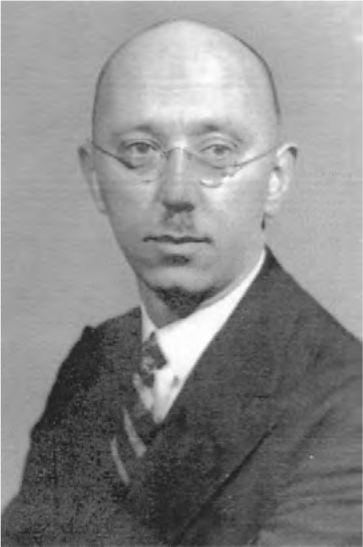
\includegraphics[height=35mm]{figs/StefanKaczmarz} \qquad 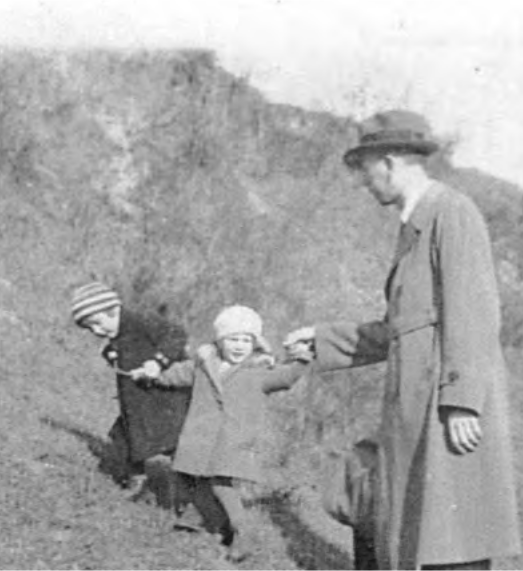
\includegraphics[height=35mm]{figs/Kaczmarz-w-2-daughters} \qquad 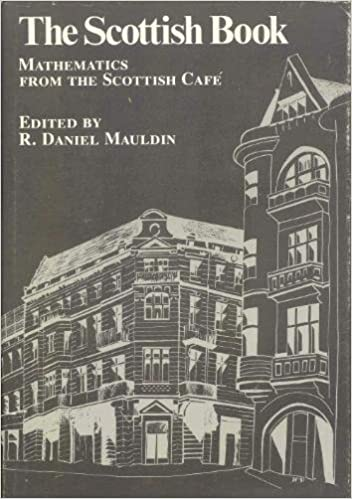
\includegraphics[height=35mm]{figs/scottish-book}
\end{center}
\end{frame}


\begin{frame}{geometric meaning}

\begin{quote}
Geometrically the algorithm means the following: The point $\bx_0$ is projected orthogonally onto the first hyperplane $H_1$; this projection is just the point $\bx_1$, which is now cast onto $H_2$, etc. The point $\bx_n$ is again cast onto $H_1$, giving the point $\bx_{n+1}$, etc. In this way, the convergence of the algorithm is easily plausible.  \hspace{18mm} {\normalfont Kaczmarz, 1937}
\end{quote}

\bigskip
\small
\begin{columns}
\begin{column}{0.4\textwidth}
\begin{itemize}
\item hyperplane $H_i$ is the set of solutions to the $i$th equation:
    $$H_i = \left\{\by\,|\,\ba_i \by = b_i\right\} \subset \RR^n$$
\item plausible because leg of a right triangle is shorter than hypotenuese!
\end{itemize}
\end{column}
\begin{column}{0.6\textwidth}
\hfill 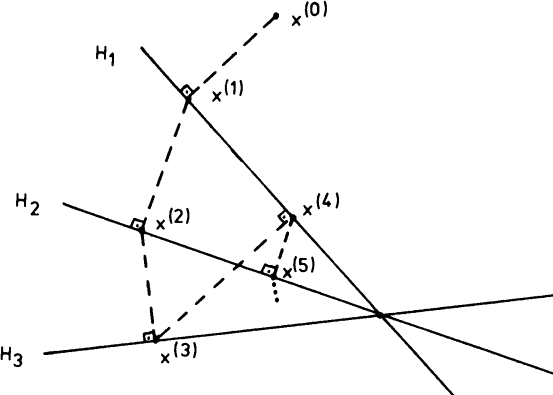
\includegraphics[width=0.8\textwidth]{figs/kaczmarz-censor.png}

\vfill
\hfill \tiny figure from Censor (1981)
\end{column}
\end{columns}
\end{frame}


\begin{frame}{geometric meaning $\implies$ formula}

\begin{itemize}
\item Kacmarz iteration is projection onto successive hyperplanes:
\begin{align*}
\bx_{k+1} &= \bx_k + c\, \ba_i^\top & &\text{update $\Delta\bx$ is orthogonal to $H_i$} \phantom{sladkjf} \\
\ba_i \bx_{k+1} &= b_i            & &\text{new iterate $\bx_{k+1}$ is in $H_i$}
\end{align*}
\item solve for $c$:
    $$c = \frac{b_i - \ba_i \bx_k}{\ba_i \ba_i^\top} \hspace{70mm}$$
\item get the formula:
    $$\bx_{k+1} = \bx_k + \frac{b_i - \ba_i \bx_k}{\|\ba_i\|^2}\, \ba_i^\top \hspace{65mm}$$
\end{itemize}

\vspace{-40mm}
\hfill 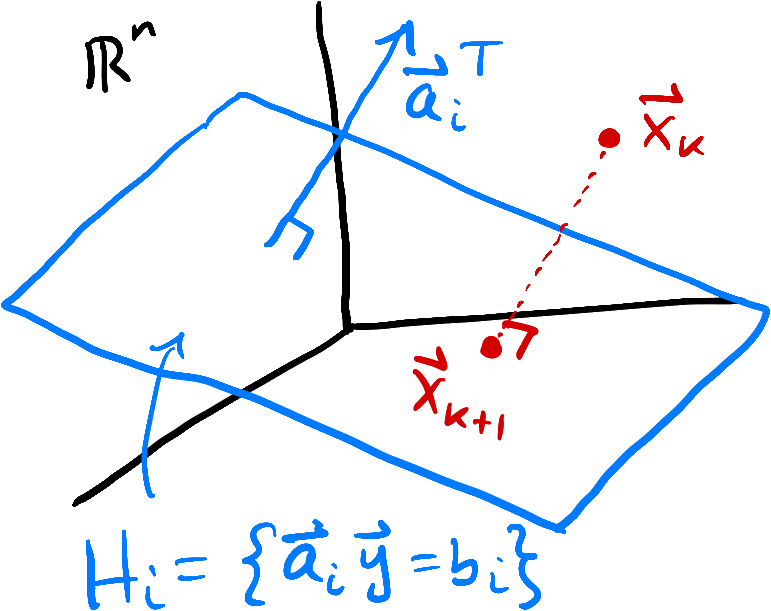
\includegraphics[width=0.53\textwidth]{figs/hyperproj.png}
\end{frame}


\begin{frame}{small hyperplane angle $\implies$ slow}

\begin{columns}
\begin{column}{0.6\textwidth}
\begin{itemize}
\item for example, this $2\times 2$ system:
\begin{align*}
5 x_1 - x_2 &= 1 \\
6 x_1 - x_2 &= 2
\end{align*}

    \begin{itemize}
    \item[$\circ$] unique solution $\bx = \begin{bmatrix} 1 & 4 \end{bmatrix}^\top$
    \item[$\circ$] condition number: $k(A) = 62.9$
    \end{itemize}
\item for most $\bx_0$, the iterates $\bx_1$, $\bx_2$,  $\bx_3$, \dots bounce back and forth between $H_1$ and $H_2$ without decent progress
\item error $\|\bx_k - \bx\|$ for 8000 iterations starting from $\bx_0 = \begin{bmatrix} -3 & -3 \end{bmatrix}^\top$ \hfill $\to$
\end{itemize}
\end{column}
\begin{column}{0.4\textwidth}
\hfill 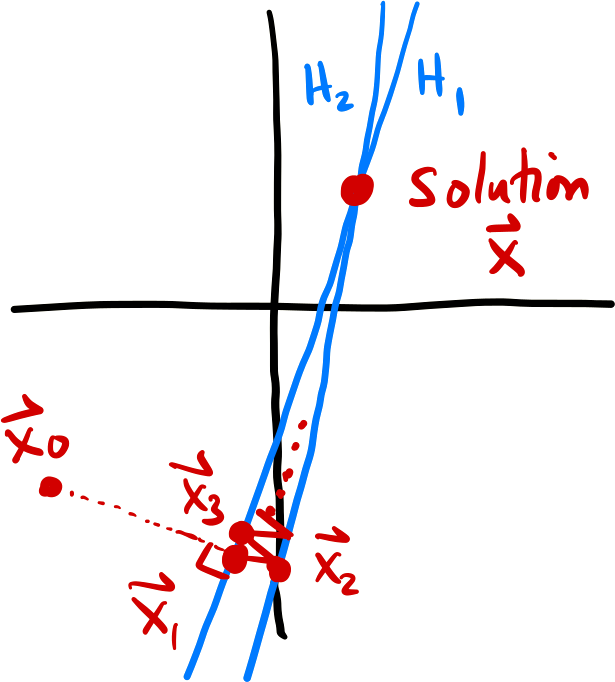
\includegraphics[width=0.9\textwidth]{figs/bad2.png}

\bigskip
\hfill 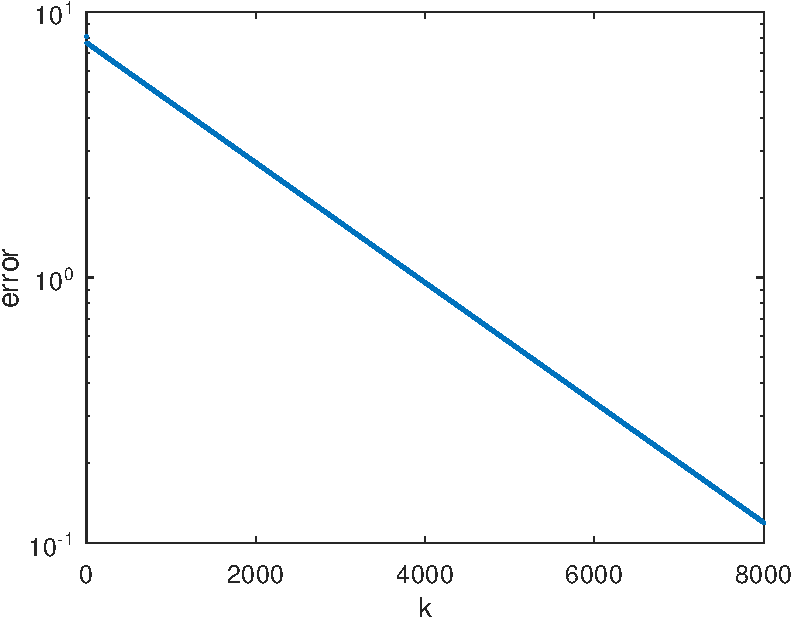
\includegraphics[width=0.9\textwidth]{figs/bad2err.pdf}
\end{column}
\end{columns}
\end{frame}


\begin{frame}{error analysis 1: reset the origin}

\begin{itemize}
\item note a solution \alert{$\bx$} is in $\bigcap H_i$
\item define vector \emph{error}\,: \, $\be_k = \bx_k - \alert{\bx}$
\item normalize the rows: \, $\balpha_i = \ba_i/\|\ba_i\|$

\vspace{-20mm}
\hfill 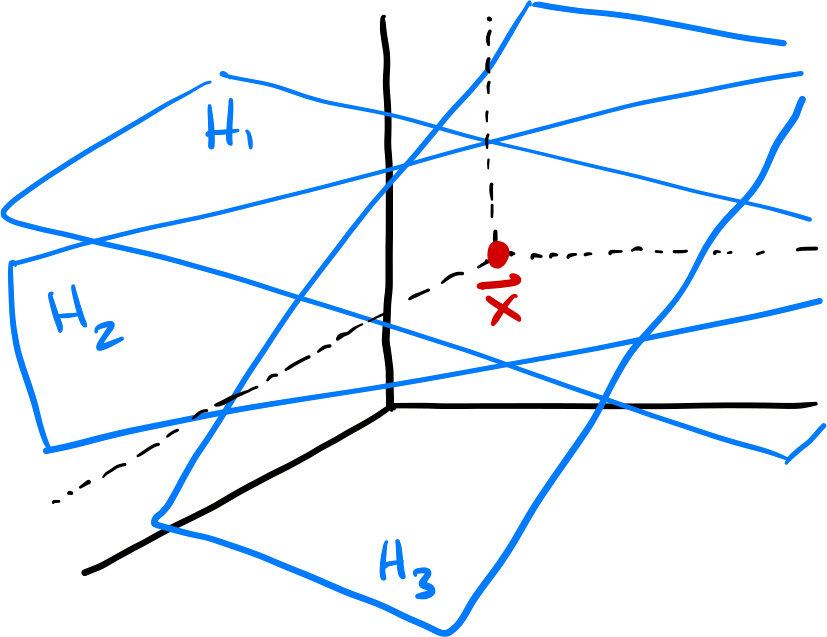
\includegraphics[width=0.4\textwidth]{figs/hyperintersect.png}

\vspace{-10mm}
\item calculate:
\begin{align*}
\bx_{k+1} &= \bx_k + \frac{b_i - \ba_i \bx_k}{\|\ba_i\|^2}\, \ba_i^\top \hspace{30mm} \\
\bx_{k+1} - \alert{\bx} &= \bx_k - \alert{\bx} + \frac{\ba_i \alert{\bx} - \ba_i \bx_k}{\|\ba_i\|}\,\frac{\ba_i^\top}{\|\ba_i\|}  \\
\be_{k+1} &= \be_k - (\balpha_i \be_k) \balpha_i^\top
\end{align*}
\item matrix $\balpha_i^\top \balpha_i$ orthogonally projects onto $\ba_i^\top$
\item each iteration projects-out $\balpha_i$: \quad $\be_{k+1} = \left(I - \balpha_i^\top \balpha_i\right) \be_k$
\end{itemize}
\end{frame}


\begin{frame}{error analysis 2: error norms decrease}

\begin{lemma}[Kaczmarz, 1937] sequence $\|\be_k\|^2$ is decreasing: \, $\|\be_{k+1}\|^2 = \|\be_k\|^2 - (\balpha_{i} \be_k)^2$
\end{lemma}

\begin{proof}
\begin{align*}
    \be_{k+1} &= \be_k - (\balpha_i \be_k) \balpha_i^\top \qquad\qquad \text{[$\gets$ previous slide]}\\
    \|\be_{k+1}\|^2 &= (\be_k - (\balpha_i \be_k) \balpha_i^\top)^\top (\be_k - (\balpha_i \be_k) \balpha_i^\top) \\
                    &= \|\be_k\|^2 - 2(\balpha_i \be_k)^2 + (\balpha_i \be_k)^2 \qed
\end{align*}
\end{proof}
\end{frame}


\begin{frame}{error analysis 3: where do errors go?}

\begin{itemize}
\item which is it?
\end{itemize}

\vspace{10mm}
\begin{columns}
\begin{column}{0.5\textwidth}
\centering
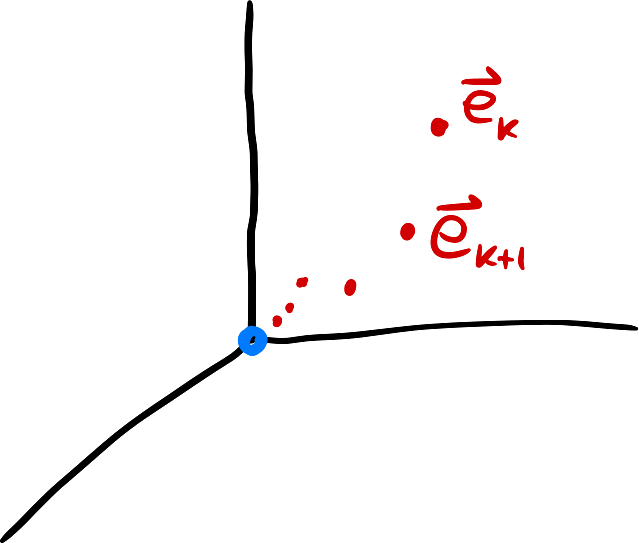
\includegraphics[width=0.85\textwidth]{figs/zero-limit.png}

\vspace{-3mm}
$\lim_k \|\be_k\| = 0$
\end{column}
\begin{column}{0.5\textwidth}
\centering
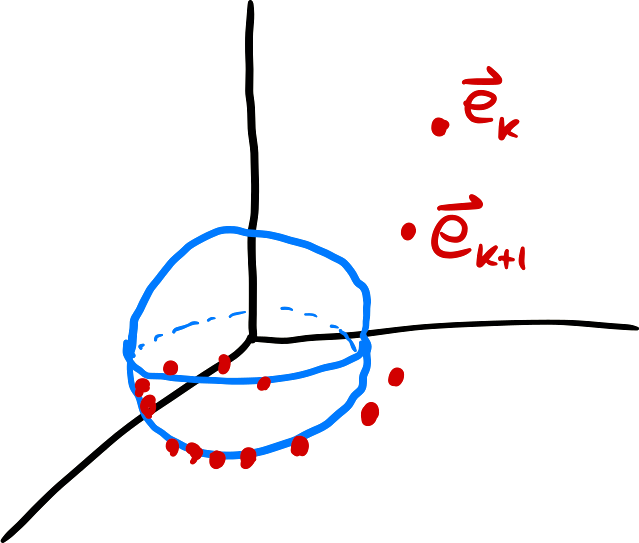
\includegraphics[width=0.85\textwidth]{figs/ball-limit.png}

\vspace{-3mm}
$\lim_k \|\be_k\| > 0$
\end{column}
\end{columns}
\end{frame}


\begin{frame}{error analysis 4: use compactness}

\begin{itemize}
\item expand a full cycle:
    $$\|\be_{(j+1)m}\|^2 \stackrel{\ast}{=} \|\be_{jm}\|^2 - (\balpha_1 \be_{jm})^2 - (\balpha_2 \be_{jm+1})^2 - \dots - (\balpha_m \be_{jm+m-1})^2$$
\item sequence $\|\be_{jm}\|^2 \ge 0$ is decreasing so the set $\{\be_{jm}\}_{j=0}^\infty \subset \RR^n$ is bounded
\item by \alert{compactness} of balls in $\RR^n$ there is a subsequence $\be_{j_\ell m}$ which converges: \quad $\ds \lim_{\ell\to\infty} \be_{j_\ell m} = \bz$

\item by continuity: $\balpha_i \be_{j_\ell m} \to \balpha_i \bz$ for each $i$
\item by $\ast$, we have $\balpha_i \be_{j_\ell m + i - 1} \to \bzero$ for each $i$
\item recalling $\be_{k+1} = \be_k - (\balpha_{i(k)} \be_k) \balpha_{i(k)}^\top$, we have, for each $i$:
    $$\|\be_{j_\ell m + i} - \be_{j_\ell m + i - 1}\| = |\balpha_i \be_{j_\ell m + i - 1}| \|\balpha_i^\top\| \to 0$$
\item by induction, for each $i$ we have:
    $$\balpha_i \bz = \lim_{\ell} \balpha_i \be_{j_\ell m} = \lim_{\ell} \balpha_i \be_{j_\ell m + i - 1} = \bzero$$
\end{itemize}
\end{frame}


\begin{frame}{theorem: always converges}

\begin{itemize}
\item from error analysis: $\balpha_i \bz = \bzero$ for each $i$ (where $\bz = \lim_\ell \be_{j_\ell m}$)
\item if $A$ has linearly-independent columns, equivalently $A\bz=\bzero$ has only one solution, then $\bz=\bzero$
\item since $\|\be_k\| = \|\bx_k - \bx\|$ decreases, the whole sequence $\{\be_k\}$ converges to zero, thus $\bx_k \to \bx$
\end{itemize}

\begin{theorem}[Kaczmarz, 1937]
If $A\, \bx = \bb$ has exactly one solution $\bx\in\RR^n$, and if $A$ has nonzero rows, then the iteration
    $$\bx_{k+1} = \bx_k + \frac{b_i - \ba_i \bx_k}{\|\ba_i\|^2}\, \ba_i^\top$$
converges: $\bx_k \to \bx$.
\end{theorem}
\end{frame}


\begin{frame}{rate of convergence?}

\begin{itemize}
\item \textbf{good}: Kaczmarz iteration always converges
\item \textbf{bad}: Kacmarz's proof gives no \emph{rate} of convergence

\medskip
\item my general impression: Kacmarz iteration does \emph{not} converge quickly compared to other iterations
\end{itemize}
\end{frame}


\begin{frame}{was Kaczmarz iteration forgotten?}

\begin{itemize}
\item historical interlude \dots
\item maybe Kaczmarz iteration is a important tool which fell through the cracks in the late 20th century?
\item not really! some Kaczmarz citations/extensions below:
\end{itemize}

\bigskip
\footnotesize
\begin{tabularx}{1.0\textwidth}{r|X} 
Tanabe (1971) & extend to overdetermined/inconsistent systems \par \\ \hline
Herman et al.~(1973) & Algebraic Reconstruction Techniques, the math of CAT scans, is really Kaczmarz iteration \par \\ \hline
McCormick (1977) & extend to nonlinear problems and Hilbert spaces \par \\ \hline
Bj\"orck \& Elfving (1979) & Kaczmarz $=$ Gauss-Seidel applied to

$\begin{bmatrix} I & - A^\top \\ 0 & A A^\top \end{bmatrix} \begin{bmatrix} \bx \\ \by \end{bmatrix} = \begin{bmatrix} \bzero \\ \bb \end{bmatrix}$ \par \\ \hline
Censor (1981) & class of extensions: ``row-action methods'' \par
\end{tabularx}
\end{frame}


\begin{frame}{iterations in linear algebra?}

\begin{itemize}
\item what iterations for $A\bx=\bb$ were known before Kaczmarz?
\item next few slides are a quick survey of \emph{classical} ($=$ \emph{simple}) and \emph{Krylov} iterations
\end{itemize}
\end{frame}


\begin{frame}{classical iterations}

\begin{itemize}
\item Richardson iteration (1911):
    $$\bx_{k+1} = \bx_k + \alpha (\bb - A \bx_k)$$

    \begin{itemize}
    \item[$\circ$] adds \emph{residual} vector $\br_k = \bb - A \bx_k$ to the current iterate
    \item[$\circ$] $A=A^\top$: is steepest descent on $\phi(\bx) = \frac{1}{2} \bx^\top A \bx - \bb^\top \bx$
    \end{itemize}
\item Jacobi iteration (1840?):
    \begin{itemize}
    \item[$\circ$] decompose $A$ into diagonal and off-diagonal: \, $A = D + L + U$
    \end{itemize}
\begin{align*}
\bx_{k+1} &= D^{-1} \left(\bb - (L+U) \bx_k\right) \\
          &= \bx_k + D^{-1} (\bb - A \bx_k)
\end{align*}
\item Gauss-Seidel iteration (1874):
\begin{align*}
\bx_{k+1} &= (D+L)^{-1} \left(\bb - U \bx_k\right) \\
          &= \bx_k + (D+L)^{-1} (\bb - A \bx_k)
\end{align*}

    \begin{itemize}
    \item[$\circ$] successive overrelaxation (1950) generalizes Gauss-Seidel
    \end{itemize}
\end{itemize}
\end{frame}


\begin{frame}{simple iterations}

\begin{itemize}
\item these classical iterations are all \alert{\emph{simple iterations}}:
    $$\bx_{k+1} = \bx_k + M^{-1} (\bb - A \bx_k)$$

    \begin{itemize}
    \item[$\circ$] $M=\alpha^{-1} I$ (Richardson), $M=D$ (Jacobi), and $M=D+L$ (Gauss-Seidel) are easy-to-invert ``approximations'' of $A$
    \item[$\circ$] simple iteration $=$ Richardson iteration applied to the \emph{preconditioned} version of the linear system
    $$M^{-1} A \bx = M^{-1} \bb$$
    \item[$\circ$] the invertible matrix $M$ is called the \emph{preconditioner matrix}
    \end{itemize}
\item much is known about simple iterations and preconditioning!
    \begin{itemize}
    \item[$\circ$] lots of software support, too
    \item[$\circ$] ask me about my PETSc book \dots but not now
    \end{itemize}
\end{itemize}
\end{frame}


\begin{frame}{simple iterations converge at a known rate}

\begin{theorem}
If $A$ is square and invertible then, for any $\bx_0$, the iteration
    $$\bx_{k+1} = \bx_k + M^{-1} (\bb - A \bx_k)$$
converges to the solution of $A\bx=\bb$ if and only if
    $$\rho(I - M^{-1}A) < 1$$
where $\rho(Z)$ is the spectral radius of matrix $Z$.
\end{theorem}

\begin{proof}  $\be_{k+1} = (I-M^{-1}A) \be_k$.  Consider eigenvalues of $I-M^{-1}A$. \end{proof}

\begin{itemize}
\item rate bound: $\|\be_{k+1}\| \le \|I-M^{-1}A\| \|\be_k\|$, tight if $M^{-1}A$ is normal
\end{itemize}
\end{frame}


\begin{frame}{does Kaczmarz converge at a linear rate?}

\begin{itemize}
\item simple iterations converge \emph{linearly} when they converge
\end{itemize}

\begin{definition} Suppose $\lim_k \xi_k = 0$ for a sequence of real numbers $\xi_k$.  Convergence is at a \emph{linear rate} if $|\xi_{k+1}| \le \lambda |\xi_k|$ for $0\le \lambda < 1$.
\end{definition}

\begin{itemize}
\item simple iteration: $\lambda=\|I-M^{-1}A\|<1$ $\implies$ linear convergence
\item I am confused about when the original cyclic Kaczmarz iteration converges at a linear rate!
    \begin{itemize}
    \item[$\circ$] it seems like it ought to be true, but
    \item[$\circ$] papers I can find don't prove it,
    \item[$\circ$] and recent literature (e.g.~Strohmer \& Vershynin, 2009) aren't helping \dots ``useful theoretical estimates for its rate of convergence are still scarce''
    \end{itemize}
\end{itemize}
\end{frame}


\begin{frame}{Krylov subspaces}

\begin{definition}[Krylov, 1931] given a square matrix $A$ and a vector $\bc$, the $k$th \emph{Krylov subspace} is
    $$\mathcal{K}_k(A,\bc) = \Span\{\bc,A\bc,A^2\bc,\dots,A^k\bc\} \subseteq \RR^n$$
\end{definition}

\begin{itemize}
\item $\mathcal{K}_k$ has dimension at most $k+1$
\item it is easy to construct $\mathcal{K}_k$ if $A$ is sparse
\end{itemize}
\end{frame}


\begin{frame}{Krylov iterations}

\begin{definition} for $A\bx = \bb$ and initial iterate $\bx_0$, with residual $\br_0=\bb-A\bx_0$, a \emph{Krylov iteration} does this:
    $$\bx_{k+1} = \argmin{\by \in \RR^n} \|\by - \bx\|_B^2 \quad \text{subject to } \bx_{k+1} \in \bx_0+\mathcal{K}_{k}(A,\br_0)$$
for some SPD matrix $B$: \quad $\|\bz\|_B^2 := \bz^\top B \bz$
\end{definition}

\begin{itemize}
\item 2 most-famous examples
    \begin{itemize}
    \item[$\circ$] \emph{conjugate gradient} (CG; 1952): for SPD $A$ use $B=A$

    \medskip
    \item[$\circ$] \emph{GMRES} (1986): for general $A$ use $B=A^\top A$
        \begin{itemize}
        \item[{\color{black} $\ast$}] $\|\by - \bx\|_B^2 = (\by - \bx)^\top A^\top A (\by - \bx) = (A\by - \bb)^\top (A\by-\bb) = \|\br_{\by}\|^2$
        \end{itemize}
    \end{itemize}
\item usually applied to a preconditioned system \, $M^{-1}A \bx = M^{-1} \bb$
\item much is known about Krylov iterations and preconditioning!
    \begin{itemize}
    \item[$\circ$] lots of software support \dots PETSc etc \dots
    \end{itemize}
\end{itemize}
\end{frame}


\begin{frame}{linear algebra iteration paradigms}

$$A\,\bx = \bb$$

\begin{enumerate}
\item \alert{simple iteration}
    $$\bx_{k+1} = \bx_k + M^{-1} \left(\bb - A \bx_k\right)$$
\item \alert{preconditioned Krylov iteration}
    $$\bx_{k+1} = \argmin{\by \in \RR^n} \|\by - \bx\|_B^2 \quad \text{subject to } \bx_{k+1} \in \bx_0 + \mathcal{K}_{k}$$
\item {\Large [does Kaczmarz fit here?]}
\end{enumerate}
\end{frame}


\begin{frame}{randomized Kaczmarz iteration}

\begin{itemize}
\item Strohmer \& Vershynin (2009) received a lot of attention
    \begin{itemize}
    \item[$\circ$] 700 citations for a \emph{J.~Fourier~An.~Appl.} article is unusual
    \end{itemize}
\item they propose and analyze an algorithm:
\end{itemize}

\begin{block}{randomized Kaczmarz iteration (RKI)}
Suppose $A\bx=\bb$, with $m\times n$ matrix $A$, $m\ge n$, has exactly one solution.  Suppose $i_k \in \{1,2,\dots,m\}$ are independent random variables with $\PP(i_k = i) \sim \|\ba_i\|^2$.  Given $\bx_0$, iterate:
    $$\bx_{k+1} = \bx_k + \frac{b_{i_k} - \ba_{i_k} \bx_k}{\|\ba_{i_k}\|^2}\, \ba_{i_k}^\top$$
\end{block}

\begin{itemize}
\item \emph{idea}: instead of cycling through rows of $A\bx=\bb$, each iteration \alert{chooses a row at random with probability proportional to $\|\ba_i\|^2$}
    \begin{itemize}
    \item[$\circ$] $\sum_i \|\ba_i\|^2 = \|A\|_F^2$ is the \emph{Frobenius norm} of the matrix
    \end{itemize}
\end{itemize}
\end{frame}


\begin{frame}{RKI converges linearly in expectation}

\begin{theorem}[Strohmer \& Vershynin, 2009]
RKI converges linearly in expectation:
    $$\EE\left(\|\bx_{k+1} - \bx\|^2\right) \le \left(1 - (\|A\|_F \|A^{-1}\|_2)^{-2}\right)\EE\left(\|\bx_k - \bx\|^2\right)$$
\end{theorem}

\begin{itemize}
\item $\kappa(A) = \|A\|_F \|A^{-1}\|_2$ is the \emph{scaled condition number}
    \begin{itemize}
    \item[$\circ$] if $k(A) = \|A\|_2 \|A^{-1}\|_2$ is the usual 2-norm condition number then $\sqrt{n} \le \kappa(A) \le \sqrt{n} k(A)$
    \end{itemize}
\item theorem says RKI expected errors converge linearly at rate
    $$\lambda = 1 - \frac{1}{\kappa(A)^2} < 1$$
\end{itemize}
\end{frame}


\begin{frame}{what does it mean?}

\begin{itemize}
\item RKI convergence rate known, unlike (?) cyclic Kaczmarz
    \begin{itemize}
    \item[$\circ$] linear convergence, but only in expectation
    \end{itemize}
\item RKI has a \alert{spectrum-based convergence rate bound}
    \begin{itemize}
    \item[$\circ$] just like simple and Krylov iterations
    \end{itemize}
\item \emph{issue} (raised immediately): the row norms $\|\ba_i\|$ should not matter in Kaczmarz iteration!
\item \emph{answer}: condition numbers have this issue already!
    \begin{itemize}
    \item[$\circ$] condition number and scaled condition number are not invariant w.r.t.~row or column scalings
    \end{itemize}
\end{itemize}
\end{frame}


\begin{frame}{paradigm: sketch-and-project}

\begin{itemize}
\item of the many papers which cite Strohmer \& Vershynin (2009), I like the following idea
\end{itemize}

\begin{block}{sketch-and-project interpretation (Gower \& Richt\'arik, 2015)}
cyclic Kaczmarz and RKI are iterations in this paradigm:
    $$\bx_{k+1} = \argmin{\by \in \RR^n} \|\by - \bx_k\|_B^2 \quad \text{subject to } S^\top A\, \by = S^\top \bb$$
\end{block}

\begin{itemize}
\item $S$ is the $m\times q$ \emph{sketch matrix}
    \begin{itemize}
    \item[$\circ$] may be randomly-generated
    \item[$\circ$] $q$ is typically small
    \end{itemize}
\item $B$ is the $n\times n$, and SPD, \emph{geometry matrix} 
    \begin{itemize}
    \item[$\circ$] determines inner product $\bx^\top B \by$ and norm $\|\cdot\|_B$ on $\RR^n$
    \end{itemize}
\end{itemize}
\end{frame}


\begin{frame}{sketch-and-project examples}

$$\bx_{k+1} = \argmin{\by \in \RR^n} \|\by - \bx_k\|_B^2 \quad \text{subject to } S^\top A\, \by = S^\top \bb$$

\begin{itemize}
\item Kaczmarz iteration choices:
\begin{align*}
S &= \be_i \quad \text{($i = (k \operatorname{mod} m) + 1$ at iteration $k$)} \\
B &= I
\end{align*}
\item randomized Kaczmarz iteration (RKI) choices:
\begin{align*}
S &= \be_i \quad \text{($i$ random from $\{1,\dots,m\}$, probability $\|\ba_i\|$)} \\
B &= I
\end{align*}
\item easy to construct many other schemes
    \begin{itemize}
    \item[$\circ$] randomized coordinate descent if $A$ SPD: $S=\be_i$, $B=A$
    \item[$\circ$] randomized block Kaczmarz: $S=I_{:R}$, $B=I$
    \end{itemize}
\end{itemize}
\end{frame}


\begin{frame}{3 paradigms for linear algebra iterations}

$$A\,\bx = \bb$$

\begin{enumerate}
\item \alert{simple iteration} \hfill {\footnotesize $\left[\,M^{-1} A\, \bx = M^{-1} \bb\,\right]$}
    $$\bx_{k+1} = \bx_k + M^{-1} \left(\bb - A \bx_k\right)$$
\item \alert{preconditioned Krylov iteration} \hfill {\footnotesize $\left[\,M^{-1} A\, \bx = M^{-1} \bb\,\right]$}
    $$\bx_{k+1} = \argmin{\by \in \RR^n} \|\by - \bx\|_B^2 \quad \text{subject to } \bx_{k+1} \in \bx_0 + \mathcal{K}_{k}$$
\item \alert{sketch-and-project iteration} \hfill {\footnotesize $\left[\,S^\top A\, \bx = S^\top \bb\,\right]$}
    $$\bx_{k+1} = \argmin{\by \in \RR^n} \|\by - \bx_k\|_B^2 \quad \text{subject to } S^\top A\, \by = S^\top \bb$$
\end{enumerate}
\end{frame}


\begin{frame}{optimization versus linear systems}

\begin{itemize}
\item recall quadratic optimization versus solving a linear system:
\begin{align*}
(i)\qquad && \bx &= \argmin{\by \in \RR^n} \frac{1}{2} \by^\top A\, \by - \bb^\top \by &&\iff & A\,\bx&=\bb \\
(ii)\qquad && \bx &= \argmin{\by \in \RR^n} \frac{1}{2} \|A\, \by - \bb\|^2 &&\iff & A^\top A\,\bx&=A^\top\bb
\end{align*}

    \begin{itemize}
    \item[$\circ$] \emph{(i)} equivalent if $A$ is square and SPD
    \item[$\circ$] \emph{(ii)} equivalent if $A$ has full column rank (thus tall $m\ge n$)
    \item[$\circ$] $A^\top A\,\bx=A^\top\bb$ are the \emph{normal equations}
    \end{itemize}
\item any connection to Kaczmarz?  of course!
\item \emph{hint}: the \emph{(ii)}  functional can be written row-wise
	$$f(\by) = \frac{1}{2} \|A\, \by - \bb\|^2 = \sum_{i=1}^m \frac{1}{2} |\ba_i \by - b_i|^2$$
\end{itemize}
\end{frame}


\begin{frame}{RKI $=$ stochastic gradient descent}

\begin{itemize}
\item decompose the least-squares objective by rows:
    $$f(\by) = \frac{1}{2} \|A\, \by - \bb\|^2 = \sum_{i=1}^m f_i(\by)$$
where $f_i(\by) = \frac{1}{2} |\ba_i \by - b_i|^2$; note $\grad f_i(\by) = (\ba_i \by - b_i) \ba_i^\top \sim \ba_i^\top$
\item \emph{stochastic gradient descent} (SGD) would choose $i$ at random and descend with step size (\emph{learning rate}) $\lambda>0$:
    $$\bx_{k+1} = \bx_k - \lambda (\ba_i \bx_k - b_i) \ba_i^\top$$
\item randomized Kaczmarz iteration (RKI) chooses $\lambda = \|\ba_i\|^{-2}$:
    $$\bx_{k+1} = \bx_k - \frac{\ba_i \bx_k - b_i}{\|\ba_i\|^2} \ba_i^\top$$
    \begin{itemize}
    \item[$\circ$] choice $\lambda = \|\ba_i\|^{-2}$ minimizes distance from $\bx_{k+1}$ to $\bx$
    \item[$\circ$] a.k.a.~\emph{exact line search}
    \end{itemize}
\end{itemize}
\end{frame}


\begin{frame}{RKI solves \emph{online} linear systems}

\begin{itemize}
\item in \emph{online optimization}, the objective pieces $f_i(\by)$ form a stream
\item surprisingly, SGD does well \dots it has a good regret bound

    \begin{itemize}
    \item[$\circ$] ask me about a talk I gave for our machine learning seminar
    \end{itemize}
\item now consider:
\end{itemize}

\begin{block}{the \emph{online linear system} problem}
$\circ$\, assume the eventual $A\bx=\bb$ is consistent

$\circ$\, a stream presents random scalar equations (rows):
    $$\ba_i \bx = b_i$$

$\circ$\, generate iterates $\bx_k$ so that $\EE\left(\|\bx_k - \bx\|^2\right)$ is small
\end{block}

\begin{itemize}
\item for RKI, S\&V (2009) say: probabilities $\sim \|\ba_i\|^2$ $\implies$
    $$\EE\left(\|\bx_{k+1} - \bx\|^2\right) \le \left(1 - (\|A\|_F \|A^{-1}\|_2)^{-2}\right)\EE\left(\|\bx_k - \bx\|^2\right)$$
\end{itemize}
\end{frame}


\begin{frame}{conclusion}

\begin{itemize}
\item I am not asserting Kaczmarz iteration is a fast solver
\item but it is:

    \begin{itemize}
    \item[$\circ$] simple and geometrically-motivated
    \item[$\circ$] always convergent
    \end{itemize}
\item the 21st century has brought it back, but with randomness:

\begin{center}
\begin{tabular}{c|c}
online optimization & online linear systems \\ \hline
SGD & RKI
\end{tabular}
\end{center}

\item next few slides, the last ones, are history and references
\end{itemize}
\end{frame}


\begin{frame}{numerical linear algebra history nugget}

\begin{itemize}
\item in first half of the 20th century, three engineers (?) gave us some of the key algorithms of practical linear algebra
\item two died as soldiers in the world wars
\end{itemize}

\bigskip
\begin{columns}
\begin{column}{0.3\textwidth}
\centering
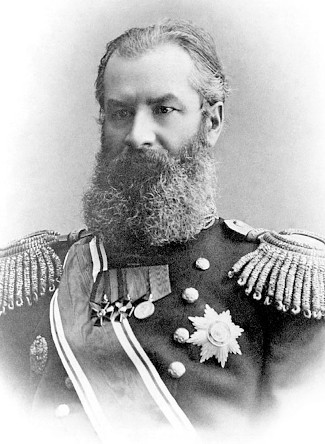
\includegraphics[height=0.5\textheight]{figs/akrylov}

\footnotesize
Alexsey Krylov

1863--1945
\end{column}
\begin{column}{0.3\textwidth}
\centering
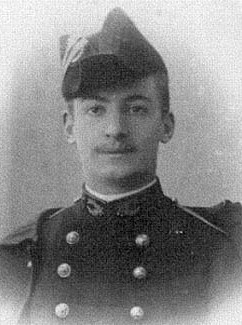
\includegraphics[height=0.5\textheight]{figs/acholesky}

\footnotesize
Andr\'e-Louis Cholesky

1875--1918
\end{column}
\begin{column}{0.3\textwidth}
\centering
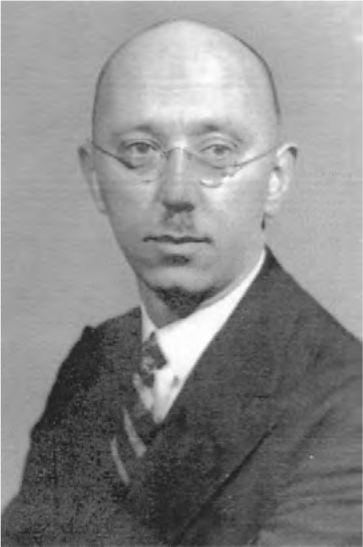
\includegraphics[height=0.5\textheight]{figs/StefanKaczmarz}

\footnotesize
Stefan Kaczmarz

1895--1939
\end{column}
\end{columns}
\end{frame}


\begin{frame}{Kaczmarz (1937):}

\begin{thebibliography}{1}
\bibitem{Kaczmarz1937}  {\footnotesize S.~Kaczmarz (1937). \textbf{Angenäherte Auflösung von Systemen linearer Gleichungen}, \emph{Bulletin International de l'Académie Polonaise des Sciences et des Lettres. Classe des Sciences Mathématiques et Naturelles. Série A, Sciences Mathématiques}, vol. 35, pp. \alert{355--357}}

\bibitem{EnglishKaczmarz1937}  {\footnotesize English translation: \textbf{Approximate Solution for Systems of Linear Equations}. \href{https://faculty.sites.iastate.edu/esweber/files/inline-files/kaczmarz_english_translation_1937.pdf}{\texttt{faculty.sites.iastate.edu/esweber/files/ inline-files/kaczmarz\_english\_translation\_1937.pdf}}}
\end{thebibliography}
\end{frame}


\begin{frame}{21st century revival references}

\begin{thebibliography}{1}

\bibitem{GowerRichtarik2015}  R.~Gower \& P.~Richt\'arik (2015).  \textbf{Randomized iterative methods for linear systems}, SIAM J.~Matrix Anal.~Appl., 36 (4): 1660--1690

\bibitem{StrohmerVershynin2009}  T.~Strohmer \& R.~Vershynin (2009). \textbf{A randomized Kaczmarz algorithm for linear systems with exponential convergence}, \emph{J.~Fourier Analysis and Appl.}, 15 (2): 262--278
\end{thebibliography}
\end{frame}


\begin{frame}{some works which cite Kaczmarz (1937)}

\begin{thebibliography}{1}
\bibitem{BjorckElfving1979} {\footnotesize A.~Bj\"orck \& T.~Elfving (1979). \textbf{Accelerated projection methods for computing pseudoinverse solutions of systems of linear equations}, \emph{BIT Numer. Math.}, 19 (2): 145--163}

\bibitem{Censor1981} {\footnotesize Y.~Censor (1981). \textbf{Row-action methods for huge and sparse systems and their applications}, \emph{SIAM Rev.}, 23 (4): 444--466}

\bibitem{Hermanetal1973} {\footnotesize G.~T.~Herman, A.~Lent, \& S.~W.~Rowland (1973). \textbf{ART: Mathematics and applications: A report on the mathematical foundations and on the applicability to real data of the algebraic reconstruction techniques}, \emph{J. Theoretical Bio.}, 42 (1): 1--32}

\bibitem{McCormick1977} {\footnotesize S.~F.~McCormick (1977). \textbf{The methods of Kaczmarz and row orthogonalization for solving linear equations and least squares problems in Hilbert space}, \emph{Indiana Univ. Math. J.}, 26 (6): 1137--1150}

\bibitem{Tanabe1971} {\footnotesize K.~Tanabe (1971). \textbf{Projection method for solving a singular system of linear equations and its applications}, \emph{Numer. Math.}, 17: 203--214}
\end{thebibliography}
\end{frame}

\end{document}
